%!TEX program = xelatex
\documentclass[11pt,class=book]{standalone}
%\usepackage[utf8]{inputenc}
\usepackage[french]{babel}
\usepackage[french]{translator}
\usepackage[T1]{fontenc}
\usepackage{fontspec}
\usepackage[table,svgnames]{xcolor}

\usepackage{pgf}
\usepackage{tikz}

\usepackage{array}
\usepackage{tabularx}
\usepackage{multirow}
\usepackage{pgf-umlsd}
\usepackage{pgfgantt}

\usetikzlibrary{shapes}
\usetikzlibrary{arrows.meta}
\usetikzlibrary{calc}

\definecolor{bg_color}{RGB}{250,250,229}

\colorlet{color1}{cyan!50}
\colorlet{color2}{red!30!green!40}
\colorlet{color3}{orange!50}
\colorlet{color4}{violet!60!blue!55}

\newganttlinktype{bartobardown}{
	\ganttsetstartanchor{south east}
	\ganttsetendanchor{north west}
	\draw [/pgfgantt/link] (\xLeft, \yUpper) -- (\xRight, \yLower);
}
\newganttlinktype{bartobarup}{
	\ganttsetstartanchor{north east}
	\ganttsetendanchor{south west}
	\draw [/pgfgantt/link] (\xLeft, \yUpper) -- (\xRight, \yLower);
}
\newganttlinktype{milestonetobardown}{
	\ganttsetstartanchor{south}
	\ganttsetendanchor{north west}
	\draw [/pgfgantt/link] (\xLeft, \yUpper) -- (\xRight, \yLower);
}
\newganttlinktype{bartomilestonedown}{
	\ganttsetstartanchor{south east}
	\ganttsetendanchor{north}
	\draw [/pgfgantt/link] (\xLeft, \yUpper) -- (\xRight, \yLower);
}


\begin{document}
	\pgfmathsetmacro\gitserverysep{50}%
	\pgfmathsetmacro\instancewidth{200}%
	\pgfmathsetmacro\instanceheight{180}%
	\pgfmathsetmacro\instancesep{120}%
	\pgfmathsetmacro\instanceinnersep{10}%
	\pgfmathsetmacro\idayshift{30}%
	\pgfmathsetmacro\idawidth{60}%
	\pgfmathsetmacro\idaheight{80}%
	\pgfmathsetmacro\idatxtyshift{20}%
	\pgfmathsetmacro\yacoidasep{5}%
	\pgfmathsetmacro\gitrepoysep{5}%
	\pgfmathsetmacro\localidbyshift{30}%
	\pgfmathsetmacro\commitsep{20}%

	\begin{tikzpicture}[x=1pt,y=1pt,>=Latex]
		\tikzset{
			database/.style={
				draw,
				cylinder,
				fill=color3,
				shape border rotate=90,
				aspect=0.25,
				text width=60,
				minimum width=50,
				minimum height=40,
				text centered
			},
			girserver/.style={
				database,
				fill=color4,
				minimum width=70,
				minimum height=50
			},
			gitrepo/.style={
				draw,
				rectangle,
				minimum width=90,
				minimum height=90,
				fill=color2
			},
			instance/.style={
				draw,
				rectangle,
				minimum width=\instancewidth,
				minimum height=\instanceheight,
				fill=bg_color
			},
			ida/.style={
				draw,
				rectangle,
				minimum width=\idawidth,
				minimum height=\idaheight,
				fill=color1
			},
			yaco/.style={
				draw,
				rectangle,
				minimum width=\idawidth-2*\yacoidasep,
				minimum height=20,
				fill=color1!30!blue
			},
			modif/.style={
				draw,
				trapezium,
				fill=color3!80!red,
				text centered,
				font=\footnotesize
			},
			commit/.style={
				draw,
				circle,
				fill=white,
				inner sep=0pt,
				minimum size=12pt
			},
			commitname/.style={
				font=\small\tt
			},
			committxt/.style={
				font=\small\tt,
				anchor=west
			},
			every path/.style={
				draw
			},
			arrow/.style={
				thick,
				red
			},
		}

		%---------------------------------
		% Instance
		\node[instance,anchor=north west] (instance) at (0,0) {};

		%---------------------------------
		% IDA & YaCo
		\node[ida,anchor=west,yshift=\idayshift] (ida) at ($(instance.west)+(\instanceinnersep,0)$) {};
		\node[anchor=north] (idatxt) at ($(ida.north)-(0,\idatxtyshift)$) {IDA};
		\node[yaco,anchor=south] (yaco) at ($(ida.south)+(0,\yacoidasep)$) {YaCo};

		%---------------------------------
		% Database & --
		\node[database,anchor=north] (codebase) at ($(ida.south)-(0,\localidbyshift)$) {IDB local};
		\draw[Square-] (codebase) -- (ida);

		%---------------------------------
		% git repo
		\node[gitrepo,anchor=east] (gitrepo) at ($(instance.east)-(\instanceinnersep,0)$) {};
		\node[anchor=north] (gitrepotxt) at (gitrepo.north) {Dépot git};
		\node[database,anchor=south] (originalidb) at ($(gitrepo.south)+(0,\gitrepoysep)$) {IDB original};
		\node[modif,anchor=south] (modif) at ($(originalidb.north)+(0,\gitrepoysep)$) {\footnotesize Modifications};
		\draw[Square-] (gitrepo.west |- yaco) -- (yaco);

		%---------------------------------
		% Sequence
		%---------------------------------

		\node[commit,green,fill=green] (c1) at (250,-160) {};
		\node[commitname] (c1txt) at (c1) {A};

		\node[commit,green,fill=green] (c2) at ($(c1)+(0,\commitsep)$) {};
		\node[commitname] (c2txt) at (c2) {B};
		\path[green] (c1) to[out=90,in=-90] (c2);

		\node[commit,green,fill=green] (c3) at ($(c2)+(0,\commitsep)$) {};
		\node[commitname] (c3txt) at (c3) {C};
		\path[green] (c2) to[out=90,in=-90] (c3);

		\node[commit,green,fill=green] (c4) at ($(c3)+(0,\commitsep)$) {};
		\node[commitname] (c4txt) at (c4) {D};
		\path[green] (c3) to[out=90,in=-90] (c4);

		%-----------------------
		\node[
			font=\small\tt,
			gray,
			above,
			anchor=south
		] (master) at (c4.north) {master};

		\node[committxt,gray] at (c1.east) {Initial commit};
		\node[committxt,gray] at (c2.east) {Modifications};
		\node[committxt,gray] at (c3.east) {Modifications};
		\node[committxt,gray] at (c4.east) {Modifications};
		\draw[dashed] (c1) -- (originalidb.east);
		\draw[dashed] (c2) -- (modif.355);
		\draw[dashed] (c3) -- (modif.0);
		\draw[dashed] (c4) -- (modif.5);

		%-----------------------
		\draw[arrow,->]  (yaco.15) to [bend left=30] (modif.180);
		\node[modif,anchor=south,fill=red] (modif) at ($(originalidb.north)+(0,\gitrepoysep)$) {\footnotesize Modifications};

		\draw[arrow,->]  (ida.300) to [bend left=40] (codebase.55);
		\node[database,anchor=north,fill=red] (codebase) at ($(ida.south)-(0,\localidbyshift)$) {IDB local};

		%-----------------------
		\node[commit,red,fill=red] (c5) at ($(c4)+(0,\commitsep)$) {};
		\node[commitname] (c5txt) at (c5) {M};
		\path[green] (c4) to[out=90,in=-90] (c5);

		\node[
			font=\small\tt,
			gray,
			above,
			anchor=south
		] (master) at (c5.north) {master};

		\draw[arrow,->]  (modif.15) to [bend left=30] (c5.180);

		%-----------------------
		\node[
			draw,
			rectangle,
			text width=200,
			anchor=east,
			inner sep=0.5,
			fill=white
		] (img) at ($(c5.west)-(30,0)$) {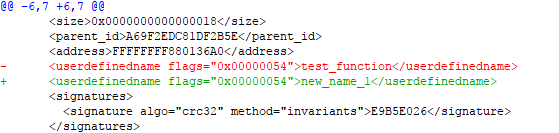
\includegraphics[width=\textwidth]{YaCo_git_diff1}};

		\draw (c5.100) -- (img.north east);
		\draw (c5.260) -- (img.south east);

		%-----------------------
		\draw[<-,ultra thick,green] ($(c1)+(0,130)$) -- ++(0,25);

		%-----------------------
		\node[commit,green!50!blue,fill=green!50!blue] (c6) at ($(c5)+(\commitsep,0)$) {};
		\node[commitname] (c6txt) at (c6) {E};
		\path[green] (c4) to[out=90,in=-90] (c6);

		\node[
			font=\small\tt,
			gray,
			above,
			anchor=south
		] (master) at (c6.north) {master};

		%-----------------------
		\node[commit,red,fill=red] (c5) at ($(c4)+(0,2*\commitsep)$) {};
		\node[commitname] (c5txt) at (c5) {M};
		\path[green] (c4) to[out=90,in=-90] (c5);

		%-----------------------
		\node[
			draw,
			rectangle,
			text width=200,
			anchor=east,
			inner sep=0.5,
			fill=white
		] (img) at ($(c6.west)-(30,0)$) {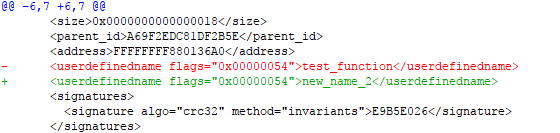
\includegraphics[width=\textwidth]{YaCo_git_diff2}};

		\draw (c6.100) -- (img.north east);
		\draw (c6.260) -- (img.south east);

		%-----------------------
		\node[commit,red,fill=red] (c7) at ($(c6)+(0,\commitsep)$) {};
		\node[commitname] (c7txt) at (c7) {M'};
		\path[green] (c6) to[out=90,in=-90] (c7);

		\node[
			font=\small\tt,
			gray,
			above,
			anchor=south
		] (master) at (c7.north) {master};

		%-----------------------
		\node[
			draw,
			rectangle,
			text width=200,
			anchor=north west,
			inner sep=0.5,
			fill=white
		] (img) at (10,-10) {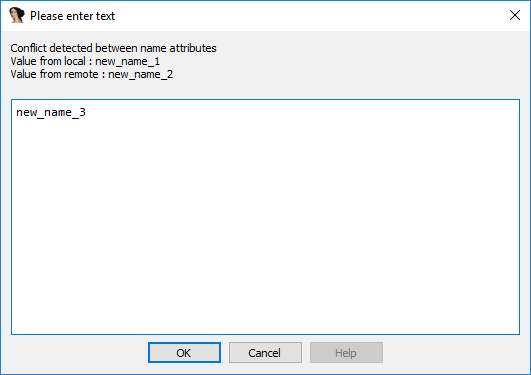
\includegraphics[width=\textwidth]{YaCo_conflict_view}};

		\draw (c7.west) -- (c7 -| img.east);

		%-----------------------
		\node[commit,green!50!blue,fill=green!50!blue] (c8) at ($(c4)+(0,\commitsep)$) {};
		\node[commitname] (c8txt) at (c8) {E};
		\path[green] (c4) to[out=90,in=-90] (c8);

		%-----------------------
		\node[commit,red,fill=red] (c9) at ($(c8)+(0,\commitsep)$) {};
		\node[commitname] (c9txt) at (c9) {M'};
		\path[green] (c8) to[out=90,in=-90] (c9);

		\node[
			font=\small\tt,
			gray,
			above,
			anchor=south
		] (master) at (c9.north) {master};

		%-----------------------
		\node[
			draw,
			rectangle,
			text width=200,
			anchor=east,
			inner sep=0.5,
			fill=white
		] (img) at ($(c9.west)-(30,0)$) {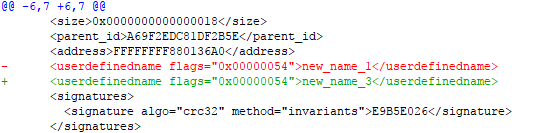
\includegraphics[width=\textwidth]{YaCo_git_diff3}};

		\draw (c9.100) -- (img.north east);
		\draw (c9.260) -- (img.south east);

		%-----------------------
		\draw[->,ultra thick,green] ($(c1)+(0,130)$) -- ++(0,25);
	\end{tikzpicture}
\end{document}
